Underwater backscatter has a mixture of many compositions, from bubbles and sand to all sorts of marine debris. It is much easier to explore the image processing theory for one backscatter composition type and later expand to cover others. Many environmental analysis fields employ systems for underwater bubble quantification to study gas seepages from the sea floor with precise outline detection and movement tracking to parameterise the overall chemical composition. Gas escape measurement and monitoring systems require high precision, extensive range, strong anti-interference, and low cost under complex underwater conditions \cite{zhangUnderwaterBubbleEscape2023}.

An accurate backscatter cancellation system must consider two main factors: (a) segmentation by isolating the bubbles from the image background and (b) determining their positions and sizes with bubble tracking in successive frames. Section \ref{bi_mv} investigates environmental analysis-related literature to discuss these two factors. A real-time approach enables predictability by knowing the exact time it takes to process each task, ensuring stability when carrying out underwater imaging missions requiring image stitching, as it is imperative to match the system processing speed to the UUV motion. Section \ref{bi_rt} begins discussing this topic with the real-time operating system (RTOS), analysing limitations and alternatives. A system to predict future positions concerning the tracked locations in a finite count of previous frames may help reduce machine-vision system complexity, considering two approaches: (a) an interpolative approach with an application of either a linear or polynomial interpolation algorithm or (b) an artificial intelligence (AI) approach, harnessing supervised machine learning (ML) methods with a potential to incorporate unsupervised methods for greater accuracy, Section \ref{bi_ps} analyses possible strategies and limitations. Finally, Section \ref{bi_bb} studies computer systems, a specialised camera sensor, a specialised light source, and concludes with discussing programming languages and libraries.

\subsection{Machine Vision for Backscatter Detection and Tracking}
\label{bi_mv}
Previous work on this project \cite{katieshepherdMachineVisionBased2023} outlines the backscatter segmentation system revolving around a simple blob detection algorithm \cite{opencvOpenCVCvSimpleBlobDetector}. A `blob' in this context refers to a group of connected pixels in a binary image \cite{theodoreWhatExactlyBlob}. The algorithm first applies several thresholds to a source image, then extracts connected pixels from and calculates their centre positions. The algorithm groups the centre positions from the set of binary images and denotes the centre position, an adjustable distance apart, that forms a group as a blob, which the algorithm uses to estimate and return the final centre positions and radii for each blob. While simple blob detection is a viable method due to computational simplicity, as \cite{katieshepherdMachineVisionBased2023} mentions, for blob detection to isolate, the blobs must share at least one property, such as size or shape. Underwater is a volatile environment where backscatter particles may be unique, so the system must account for varying backscatter properties.

The paper in \cite{thomanekAutomatedGasBubble2010} presents the design of a novel method for automated gas bubble imaging. In contrast to the work in \cite{katieshepherdMachineVisionBased2023}, this paper employs the Canny edge detection algorithm \cite{cannyComputationalApproachEdge1986} for greyscale images to overcome the limitations of blob detection. The Canny filter compares the value of each pixel relative to its neighbours, so when the gradient between two adjacent pixels is higher than a certain threshold, the algorithm sets the bordering pixel to a value of binary `1', otherwise `0', resulting in the formation of edges around objects. The paper compares the Canny segmentation approach with simple thresholding (blob detection approach), an illustration in Figure \ref{fig:bubble_segment_canny}, and deduces Canny as more accurate for segmentation, even in inhomogeneously illuminated areas. However, the disadvantages of Canny, as stated in \cite{thomanekAutomatedGasBubble2010}, are the drastic increase in computing time and the requirement for implementing morphological techniques to account for the growing or shrinking of bubbles during segmentation. However, it has been 14 years since the publication of this paper, and the computational power of computers nowadays should handle the Canny workload easily. While this paper explores methodologies perfect for a starting point, it does focus more on the system construction and quantifying gas flux measurements, thus skipping some information on vital aspects such as how the bubbles were perfectly highlighted after Canny in Figure \ref{fig:bubble_segment_canny}, one can assume they are using logic to fill closed loop edges.

\begin{figure}[h]
    \centering
    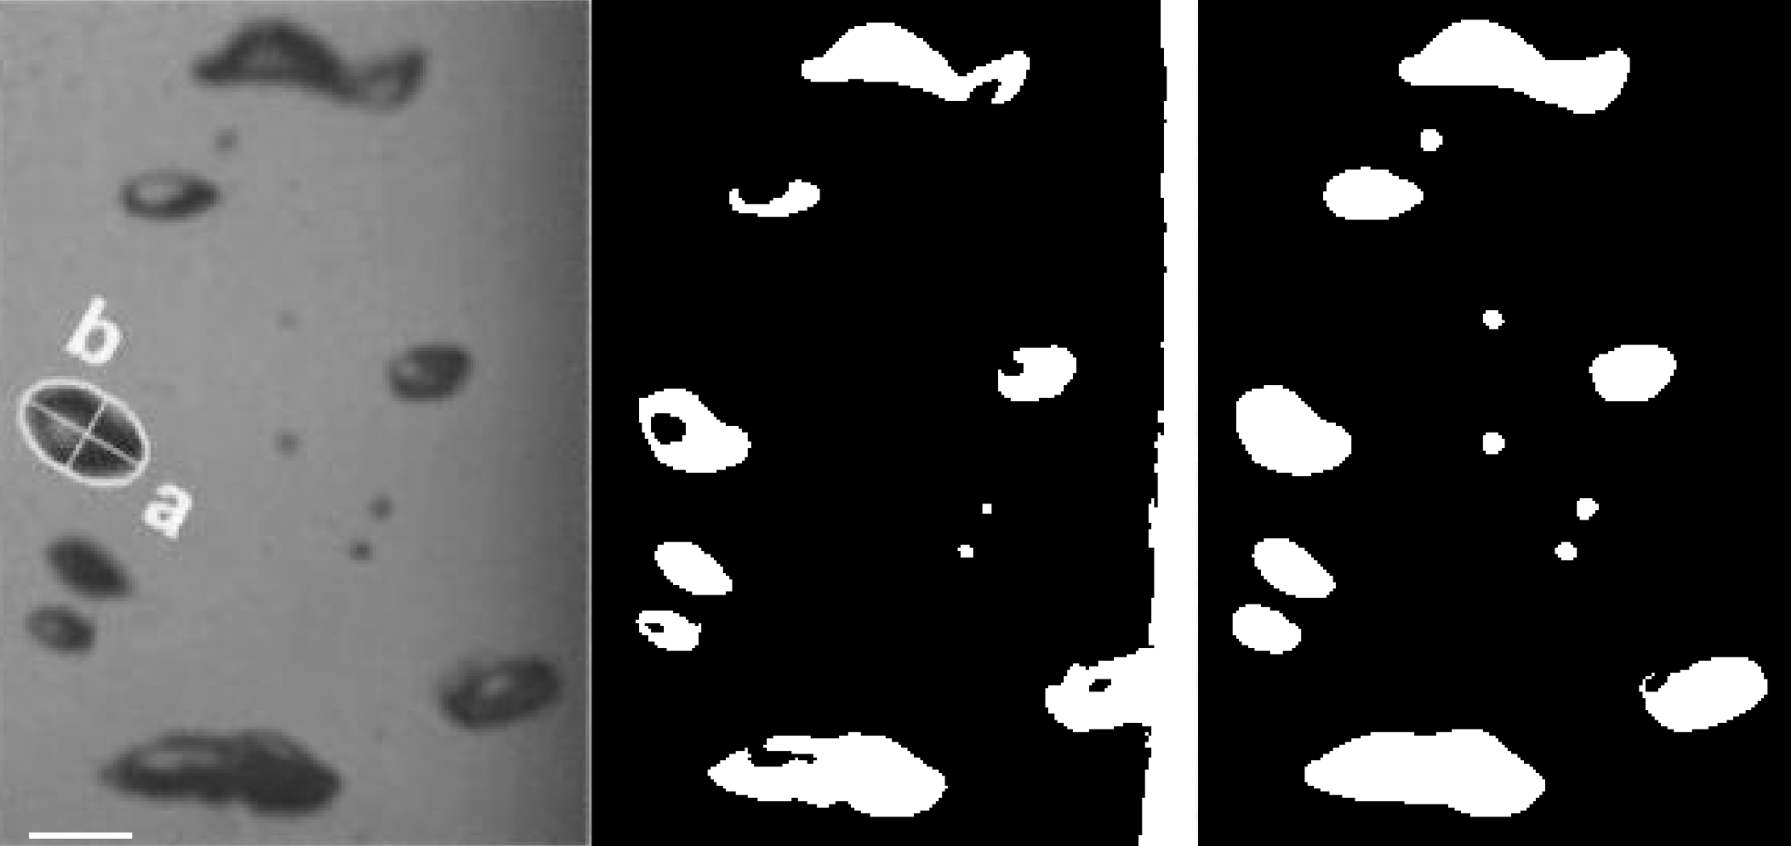
\includegraphics[width=0.35\textwidth]{assets/bubble-segmentation-canny-thresholding.png}
    \caption{An illustration from the paper in \cite{thomanekAutomatedGasBubble2010} showing the original input in the left-most image, bubble segmentation using a simple thresholding method in the middle, and bubble segmentation using Canny in the right-most image.}
    \label{fig:bubble_segment_canny}
\end{figure}

The work in \cite{zelenkaGasBubbleShape2014} expands on this Canny-based system with the motivation to derive more stable algorithms tackling the sporadical false detection characteristic of the Canny algorithm, introducing methods for precise bubble stream quantification and accurate bubble elliptical fitting with snake-based methods, where a snake is an energy-minimising spline guided by external constraint forces and influenced by image forces that pull it towards features such as lines and edges, and the Covariance Matrix Adaptation - Evolution Strategy (CMA-ES) optimisation algorithm \cite{hansenEvaluatingCMAEvolution2004}. Although false positive detections due to an unstable algorithm are not detrimental to the nature of this project, they will result in system inaccuracies, which may affect imaging quality. In an underwater environment where lighting conditions are highly variable, it is worth considering the Canny-based approach in \cite{zelenkaGasBubbleShape2014} as a benchmark and expanding with a snake method implementation, as this method achieves the highest decision rate compared to the others, illustrated in Figure \ref{subfig:zelenka_compare}, achieving an 89.7\% decision rate, a 12.4\% advantage over the standard Canny system.

\begin{figure}[h]
    \centering
    \begin{subfigure}{.30\textwidth}
        \centering
        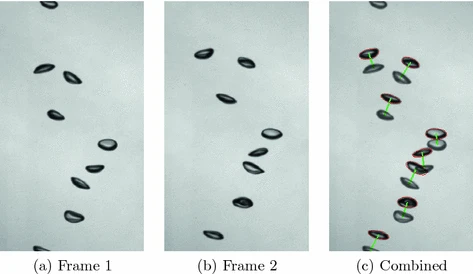
\includegraphics[width=1\linewidth]{assets/zelenkaGasBubbleShape2014-movement_tracking.png}
        \caption{}
        \label{subfig:zelenka_tracking}
    \end{subfigure}
    \qquad
    \begin{subfigure}{.45\textwidth}
        \centering
        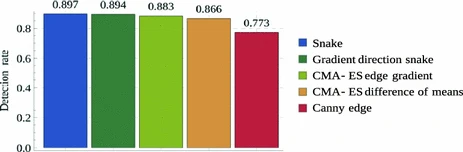
\includegraphics[width=1\linewidth]{assets/zelenkaGasBubbleShape2014-bubble-detection-methods-comparison.png}
        \caption{}
        \label{subfig:zelenka_compare}
    \end{subfigure}
    \caption{From \cite{zelenkaGasBubbleShape2014}: (a) illustration of the movement of bubbles in between two frames at 100 fps. The combination shows frames 1 and 2 with the bubble detection in frame 2 in red and matching bubbles connected in green, (b) a graph comparing the detection rates for several selected methods on a high-quality GoPro image sequence with manual ground truth on 20 images.}
    \label{fig:zelenka}
\end{figure}

The work in \cite{thomanekAutomatedGasBubble2010} also proposes a method for bubble tracking using the `least distance rule', which is the realisation that the distance a bubble travels in two successive frames is smaller than the distance to its closest neighbour. This assumption, although not valid for overlapping bubbles, very high bubble concentrations, and cases where the travel distance exceeds the neighbouring bubble distances, enables a computationally simple method for calculating positions in successive frames and the bubble rise velocity from the sea floor. Reiterating the previously mentioned point regarding the increased computational power in computers nowadays, I don't think this assumption is a fair trade-off since backscatter, especially the type forming from bubbles, can be highly concentrated, overlapping, and fast-moving due to the UUV propellors. The paper in \cite{zelenkaGasBubbleShape2014} proposes a new method for tracking bubbles using a Kalman filter \cite{kalmanNewApproachLinear1960} to predict the bubble position in a subsequent frame from detection, employing the Hungarian method \cite{kuhnHungarianMethodAssignment1955} for the minimum weighted matching of the predicted positions and the new detection of bubble positions. Figure \ref{subfig:zelenka_tracking} illustrates the system in \cite{zelenkaGasBubbleShape2014}. While it is unclear whether the Kalman filter-based method is resilient to the limitations of the `least distance rule', the paper \cite{zelenkaGasBubbleShape2014} does confirm a highly reliable tracking.

\subsection{Real-time Systems}
\label{bi_rt}
The previous work on this project in \cite{katieshepherdMachineVisionBased2023} addressed the need for a real-time operating system (RTOS). An RTOS enables the compliance of a `hard' real-time system, where there is a guarantee of the maximum time a task requires for completion. While there are RTOS products for general-purpose computer systems, they involve many limitations requiring circumvention compared to a general-purpose OS such as Linux, drastically increasing development times and resulting in a much more complicated system due to the bare-metal knowledge requirement, thus not being the best option for this project.

In Linux, when a task in user space, which is a set of locations where normal user processes run (i.e., everything other than the kernel) \cite{nlightnfotisAnswerWhatDifference2013}, is interrupted, and if the interrupt handler can wake up another task, the scheduler will schedule this task as soon as the interrupt handler returns in a pre-emptive manner. However, many sections in kernel space, which is the location where the code and data of the kernel are stored and executed under \cite{nlightnfotisAnswerWhatDifference2013}, do not support pre-emption due to the presence of spinlocks, which are non-blockable and non-sleepable programmatical loops to protect critical sections of code, pre-emption logic falls apart when a user space task calls a kernel-specific function, thus accepting a promotion to kernel space as it receives an interrupt.

Figure \ref{fig:bootlin_flow}, from the training material in \cite{bootlinUnderstandingLinuxRealtime2024}, illustrates this issue of user space task promotions to kernel space, with kernel-based spinlocks resulting in an unpredictable jitter, denoted by the green question mark. Aside from the kernel space incompatibility, Linux already supports user space pre-emption with task priority-based real-time scheduling to allow for an RTOS. The PREEMPT-RT is a kernel patch that aims to make all kernel-space code preemptible and deterministic.

\begin{figure}[h]
    \centering
    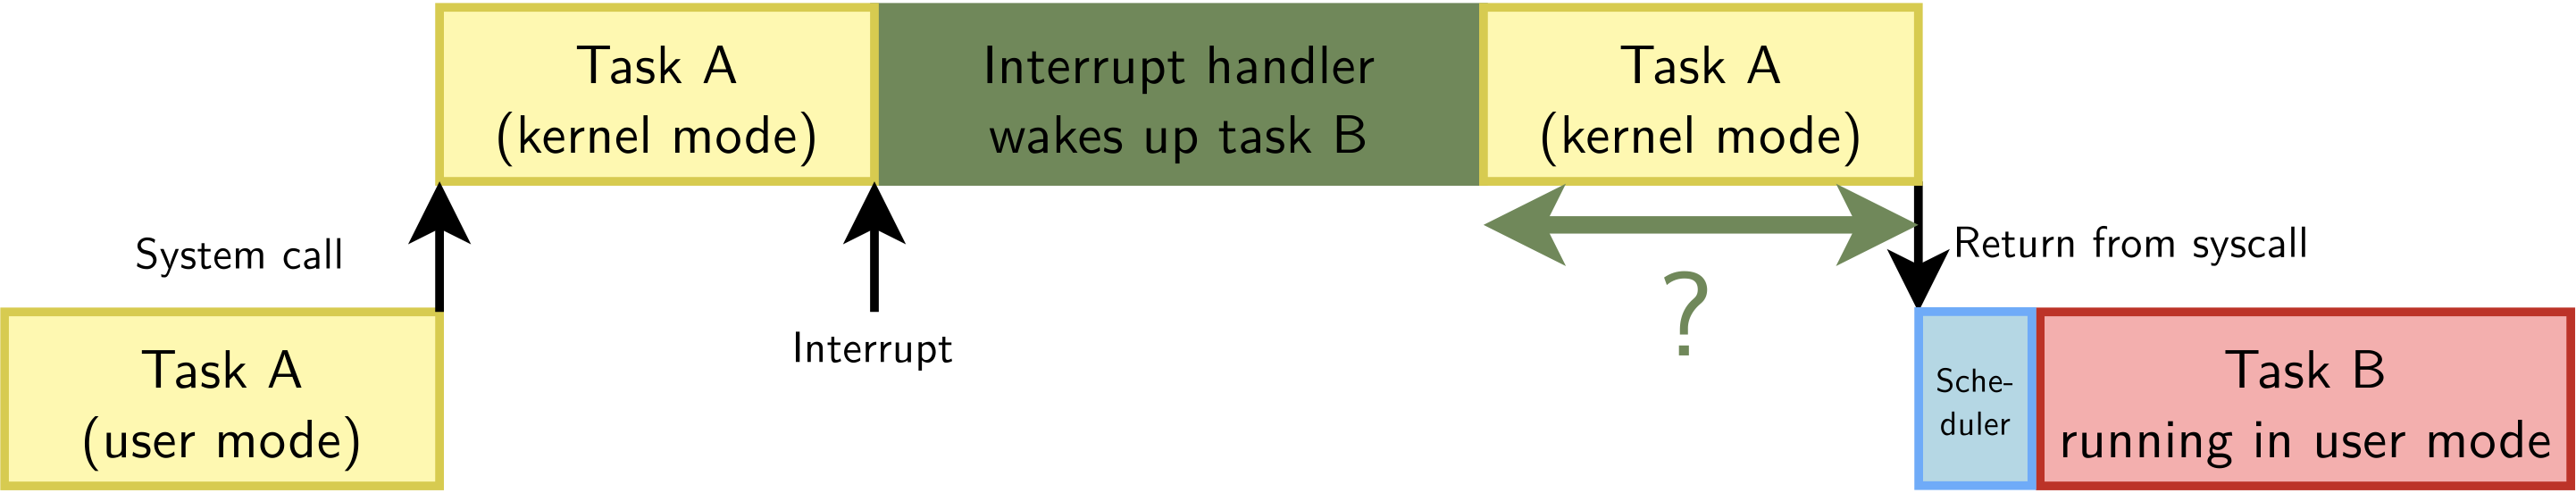
\includegraphics[width=0.9\textwidth]{assets/bootlin-interrupt-flow.png}
    \caption{Illustration by \cite{bootlinUnderstandingLinuxRealtime2024} of the interrupt flow within two tasks, one in kernel space and another in user space.}
    \label{fig:bootlin_flow}
\end{figure}

Although insufficient to convert Linux into a `hard' RTOS, as the material in \cite{bootlinUnderstandingLinuxRealtime2024} confirms, the PREEMPT-RT patch is a step in the correct direction to minimise task switching latencies. The PREEMPT-RT patch provides the best balance between low system complexity and maximum jitter prevention, making it the ideal choice to implement in this project. The blog post in \cite{maurorivaRaspberryPi4B2019}, which details the installation steps for the PREEMPT-RT kernel patch in a Raspberry Pi 4 Linux system, quantifies my earlier statement. Using the RT-Tests, a test suite that contains programs to test various real-time Linux \cite{costashulRTTests2023}, measures the latency reduction with the kernel modification, the blog post \cite{maurorivaRaspberryPi4B2019} draws comparisons with the non-RT kernel. The Cyclictest, part of RT-Tests, accurately and repeatedly measures a thread's intended wake-up time and when it wakes up to provide statistics about the system's latencies, measuring latencies in real-time systems caused by the hardware, the firmware, and the operating system \cite{costashulCyclictest2023}. Figure \ref{fig:lemariva_latency} shows the maximum latency measurement with the standard kernel was 301 us, while the PREEMPT-RT kernel was 93 us, thus confirming a 3.23x latency reduction using the kernel patch.

\begin{figure}[h]
    \centering
    \begin{subfigure}{.34\textwidth}
        \centering
        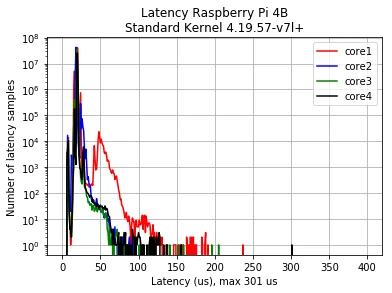
\includegraphics[width=1\linewidth]{assets/lemariva-std-kernel-latency.png}
        \caption{}
        % \label{subfig:std_kernel_latency}
    \end{subfigure}
    \qquad
    \begin{subfigure}{.34\textwidth}
        \centering
        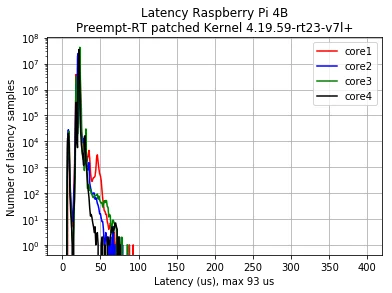
\includegraphics[width=1\linewidth]{assets/lemariva-rt-kernel-latency.png}
        \caption{}
        % \label{subfig:rt_kernel_latency}
    \end{subfigure}
    \caption{Illustration from \cite{maurorivaRaspberryPi4B2019} showing the latency measurements following a Cyclictest execution from the RT-Tests suite for (a) the standard Linux RPi kernel and (b) the PREEMPT-RT patch Linux RPi kernel.}
    \label{fig:lemariva_latency}
\end{figure}


\subsection{Research into Predictive Systems}
\label{bi_ps}
Following the bubble segmentation theory, using the Canny edge detection with a bubble elliptical fitting method, such as the snake, should result in a rough outline of the bubbles. From this outline, an elliptical best-fit technique can estimate the bubble shape and characteristics, such as orientation and axis, as proposed in \cite{thomanekAutomatedGasBubble2010} and illustrated in Figure \ref{fig:bubble_segment_canny} in the left-most image with the bubble bordered by a while ellipse with `a' and `b' denoting the dimensions. The blog post in \cite{steveeddinsEllipseVisualizationRegionprops2015} exemplifies this technique using the MATLAB `regionprops' function \cite{MeasurePropertiesImage}, which automatically determines the properties of each contiguous white region that is 8-connected \cite{rayryengAnswerExplanationMatlab2014}. This technique allows for computing the exact centroid position of bubble detection. This function is not limited to MATLAB, as there are implementations for other programming languages, such as Python \cite{MeasureRegionProperties}. An assumption for this technique is the 8-connected region compliance, where from a given pixel, you can get to any other pixel in the region by a series of 8-way moves (up, down, left, right, up-left, up-right, down-left, down-right) \cite{CourseNoteComputer}. Therefore, edges that are not closed loops will not be compatible. However, given the highly optimised methods to improve the Canny edge detection technique, it is theoretically unlikely to have many open-looped detections.

By considering just the centroid of each bubble, we can reduce dimensionality, thus reducing complexity, in contrast to computing each pixel of a detected bubble border. This optimisation is crucial for efficiently storing and processing bubble positions across multiple frames. Predicting future bubble positions of the bubbles that travel in a straight line is straightforward with linear interpolation. Predicting non-straight moving bubble positions is possible by considering non-linear interpolation with spline curves. Dimensionality reduction is especially vital when considering machine learning approaches to aid in more accurate predictions and quick processing. A possible machine learning approach is with classifiers, which are algorithms that automatically order or categorise data into one or more of a set of ``classes" \cite{tobiasgeislermesevageMachineLearningClassifiers2020}. The biggest challenge with an ML approach is generating ground-truth data for training the models since it is very labour-intensive to manually inspect each frame in example footage to select bubble locations. However, an elliptical best-fit technique can speed up this process. The project must research these methodologies in more detail.

\subsection{System Building Blocks}
\label{bi_bb}
\subsubsection{Computing Platforms}
The website in \cite{dev22adminGPUVsFPGA2023} mentions Field Programmable Gate Arrays (FPGAs) to be well-suited for computationally intensive image processing tasks, due to hardware parallelism, and well-known for their low latency, making them suitable for applications where real-time image processing is critical. FPGAs are semiconductor devices based around a matrix of configurable logic blocks (CLBs) connected via programmable interconnects, enabling the hardware reprogramming to desired application or functionality requirements after manufacturing \cite{WhatFPGAField}. Unlike FPGAs, CPUs compute sequentially, breaking algorithms into operations by sequence, thus limiting execution to one operation at a time \cite{alexliangBoostingMachineVision2016}. Despite many highly efficient intellectual property (IP) cores for re-usable FPGA-based logic to accelerate FPGA development, the development and prototyping times will increase due to the low-level hardware intricacies. Furthermore, FPGAs are, on average, much more expensive than traditional CPU-based computers. The Raspberry Pi (RPi) company has been designing high-performance, low-cost, general-purpose, single-board and modular computers built on the Arm architecture and running the Linux operating system since 2012 \cite{raspberrypiRaspberryPiUs}. The regular RPi product series is perfect for a non-FPGA, CPU-based route for quick and easy development and deployment. The newer RPi models implement various features such as built-in RAM up to 8GB, a dedicated GPU and video decoder, HDMI output interfaces, dual-band WiFi with Bluetooth capabilities, a Gigabit Ethernet interface, USB 3.0 and 2.0 ports, MIPI-compatible serial interfaces for cameras and displays, and an array of 40 GPIO pins \cite{raspberrypiltdBuyRaspberryPi, raspberrypiltdBuyRaspberryPia}.

\subsubsection{Specialised Light Source}
A Digital Light Processing (DLP) projector is vital for projecting backscatter-cancelling light patterns. The DLP chipset, created by Larry Hornbeck of Texas Instruments in 1987, consists of a Digital Micromirror Device (DMD) that houses millions of reflective aluminium mirrors, usually a few microns wide \cite{DigitalLightProcessing2024, HowDoesDLP}. The DMD is a Micro-Opto-Electro-Mechanical System (MOEMS) Spatial Light Modulator (SLM) that uses digital signals to control the angle of each mirror, enabling the modulation and attenuation of an incident light beam \cite{DLP4500DigitalMicromirror}. As \cite{HowDLPProjector} explains the intricacies and Figure \ref{fig:dmd_dlp} illustrates, a DLP projector implements this specialised technology: The beam of a high-intensity white lamp directs into a spinning colour-tinted lens wheel consisting of red, green, and blue, and a clear lens for a white lamp pass-through. An internal lens diffracts the coloured beam incident into the DMD, with the angle and time spent in each microscopic mirror controlling the individual pixel colour and intensity. The DMD directs the desired beams of each pixel into the diffraction lens to exit the projector. The DMD will not actuate for undesired pixel beams, thus sending the beam into a light-absorbent region to prevent leakage and image distortion.

\begin{figure}[h]
    \centering
    \begin{subfigure}{.3\textwidth}
        \centering
        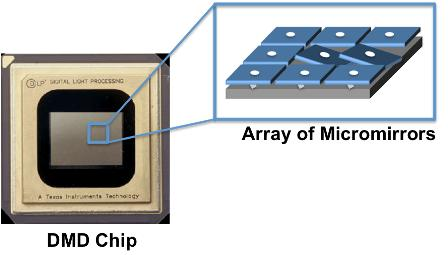
\includegraphics[width=1\linewidth]{assets/dmd-chip.jpg}
        \caption{}
        % \label{subfig:dmd_chip}
    \end{subfigure}
    % \hfill
    \qquad
    \begin{subfigure}{.35\textwidth}
        \centering
        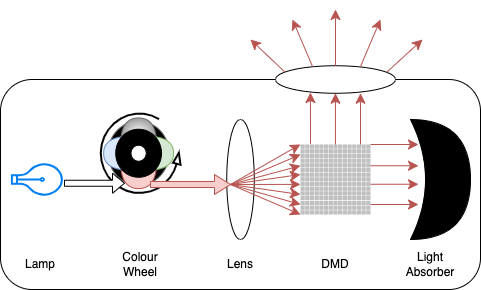
\includegraphics[width=1\linewidth]{assets/dlp-projector.png}
        \caption{}
        % \label{subfig:dlp_projector}
    \end{subfigure}
    \caption{(a) An illustration of the microscopic mirror array within a DMD chip \cite{HowDoesDLP}. (b) A cross-section illustrating the internals of an example projector utilising DLP technology.}
    \label{fig:dmd_dlp}
\end{figure}

\subsubsection{Specialised Camera Sensor}
The cameras in most traditional and consumer-grade electronic devices, such as phones, all employ a CMOS sensor with a rolling shutter and is insufficient for use in this project when capturing fast-moving backscatter particles. While these sensors are smaller and much cheaper, they cause distortion effects when capturing fast-moving subjects due to their line-by-line scan image-capturing characteristic. The article in \cite{updatedWhatGlobalShutter2021} explains: Instead of having pixels from the top of the sensor switch on and work its way down like a scan, the global shutter sensor takes a snap of the scene using all of the pixels all at once. Figures \ref{subfig:rs_timeline} and \ref{subfig:gs_timeline} illustrate the differences in image capture, and Figure \ref{subfig:rs_vs_gs} illustrates the drastic differences in each shutter type. The Raspberry Pi company produces a global shutter camera featuring a 1.6MP Sony IMX296 sensor, with plug-and-play compatibility with RPi computers \cite{raspberrypiltdBuyRaspberryPib}.

\begin{figure}[h]
    \centering
    \begin{subfigure}{.32\textwidth}
        \centering
        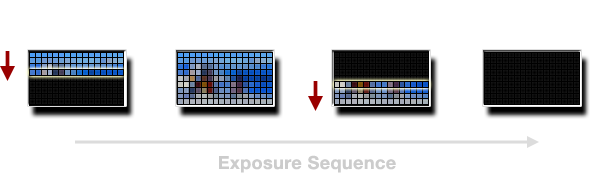
\includegraphics[width=1\linewidth]{assets/rolling-shutter-timeline.png}
        \caption{}
        \label{subfig:rs_timeline}
    \end{subfigure}
    \hfill
    \begin{subfigure}{.32\textwidth}
        \centering
        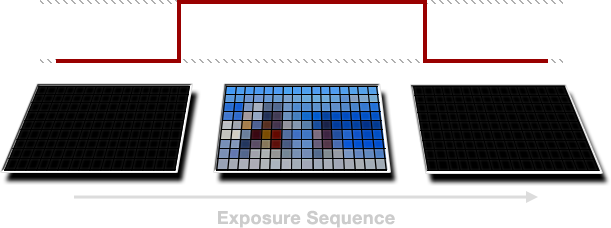
\includegraphics[width=1\linewidth]{assets/global-shutter-timeline.png}
        \caption{}
        \label{subfig:gs_timeline}
    \end{subfigure}
    \hfill
    \begin{subfigure}{0.32\textwidth}
        \centering
        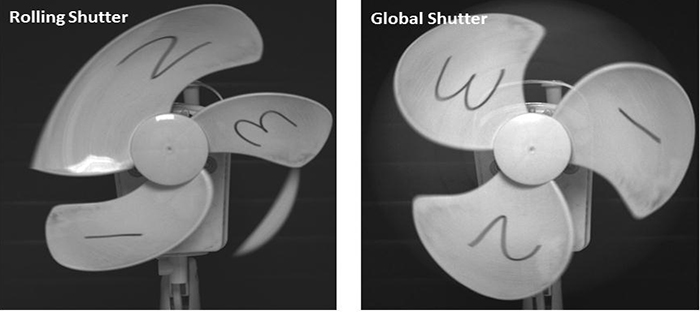
\includegraphics[width=0.7\textwidth]{assets/rolling-vs-global-shutter.jpeg}
        \caption{}
        \label{subfig:rs_vs_gs}
    \end{subfigure}
    \caption{(a) An image capture timeline of a rolling shutter sensor, (b) An image capture timeline of a global shutter sensor \cite{reddigitalcinemaGlobalRollingShutters}, (c) The distortion in the image capture of a spinning fan due to a rolling shutter, compared to a non-distorted capture from a global shutter \cite{RollingShutterVs}.}
    \label{fig:rs_vs_gs}
\end{figure}

\subsubsection{The Python Programming Language and OpenCV}
This project requires efficient machine-vision implementations and an intuitive programming language for fast development. OpenCV is an open-source computer vision and machine learning software library with over 2500 optimised algorithms, including a comprehensive set of classic and state-of-the-art computer vision and machine learning algorithms \cite{opencv}. Although native to C++, OpenCV features interfaces for Python, Java and MATLAB, ensuring compatibility vast platforms. OpenCV targets real-time vision applications by taking advantage of CPU accelerators, such as MMX and SSE instructions for parallel data processing, and GPU accelerators. OpenCV presents simple and high-level wrappers for advanced computer vision algorithms and tools to drastically reduce development and prototyping duration with little performance trade-off, vital to this project. The Python programming language presents an easy-to-read and write syntax and great debugging possibilities.
